% 导言区
\documentclass{ctexart} % ctexbook ctexrep/

\usepackage{ctex}
% 导言区:\usepackage{praphicx}
% 语法:\includegraphics[选项]{文件名}
% 格式:EPS,PDF,PNG,JPEG,BMP
\usepackage{graphicx}
\graphicspath{{figures/},{pics/}} % 图片在当前目录下的 figures 目录

% 正文区
\begin{document}
    \LaTeX{}中的插图

    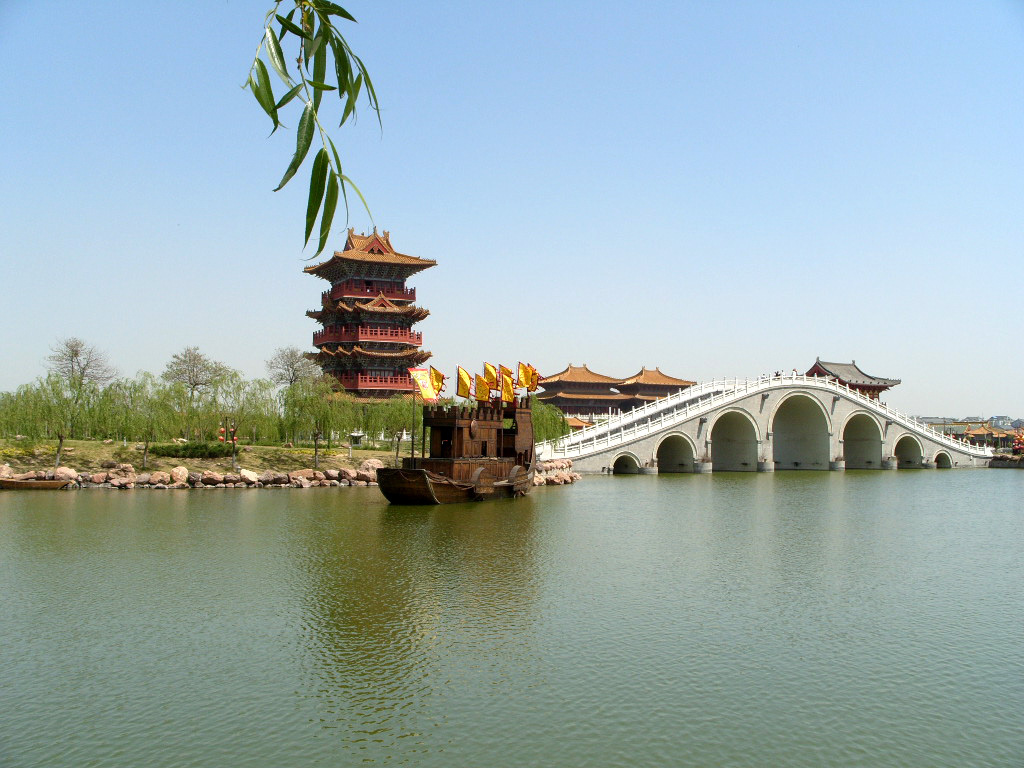
\includegraphics[width=2cm]{timg}
    
    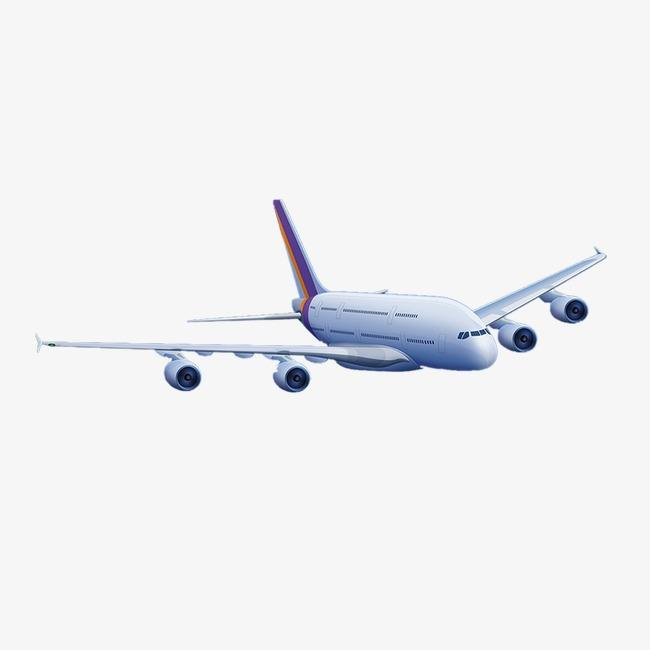
\includegraphics[width=2cm]{figures/timg1.jpg}
    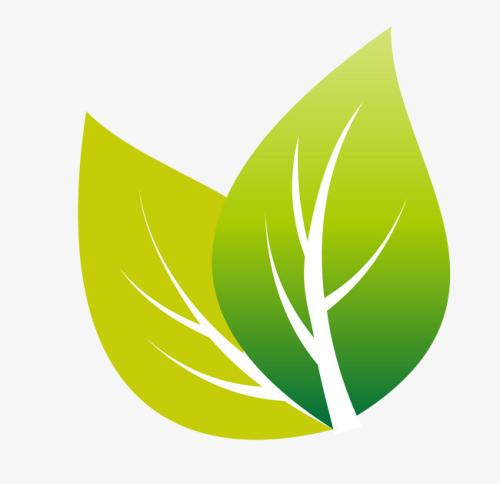
\includegraphics[width=2cm]{pics/123.jpg}

\end{document}

% %%% Local Variables:
% %%% mode: latex
% %%% TeX-master: t
% %%% End:

% \documentclass[doctor]{thuthesis}
% % \documentclass[%
% %   bachelor|master|doctor, % mandatory option
% %   xetex|pdftex|dvips|dvipdfm, % optional
% %   secret,
% %   openany|openright,
% %   arialtoc,arialtitle]{thuthesis}

% % 所有其它可能用到的包都统一放到这里了,可以根据自己的实际添加或者删除。
% \usepackage{thutils}

% % 你可以在这里修改配置文件中的定义,导言区可以使用中文。
% % \def\myname{薛瑞尼}

% \begin{document}

% % 定义所有的eps文件在 figures 子目录下
% \graphicspath{{figures/}}


% %%% 封面部分
% \frontmatter
% \input{data/cover}
% \makecover

% % 目录
% \tableofcontents

% % 符号对照表
% \input{data/denotation}


% %%% 正文部分
% \mainmatter
% \include{data/chap01}
% \include{data/chap02}


% %%% 其它部分
% \backmatter

% % 本科生要这几个索引,研究生不要。选择性留下。
% \makeatletter
% \ifthu@bachelor
%   % 插图索引
%   \listoffigures
%   % 表格索引
%   \listoftables
%   % 公式索引
%   \listofequations
% \fi
% \makeatother


% % 参考文献
% \bibliographystyle{thubib}
% \bibliography{ref/refs}


% % 致谢
% \include{data/ack}

% % 附录
% \begin{appendix}
% \input{data/appendix01}
% \end{appendix}

% % 个人简历
% % \include{data/resume}
% \end{document}